\section{Wstęp}
\indent

Elektrokardiografia to zabieg diagnostyczny, który jest wykorzystywany głównie
do rozpoznawania chorób serca~\cite{EKG-Wiki}. Polega ona na rejestracji
czynności elektrycznej mięśnia sercowego przedstawianej następnie w~postaci
krzywej EKG. Przykładowy sygnał przedstawiony jest na rysunku~\ref{fig:pqrst}.
\begin{figure}[!ht]
    \centering
    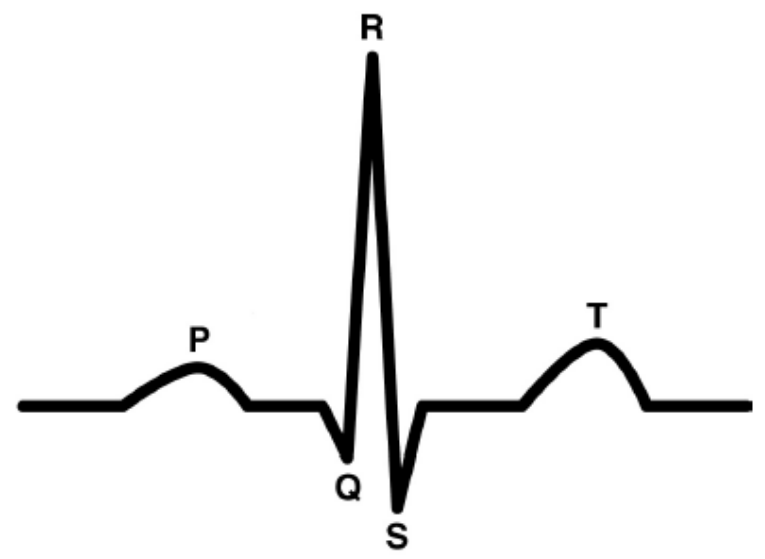
\includegraphics[width=0.5\textwidth]{../img/pqrst.png}
    \caption{Sygnał EKG}
    \label{fig:pqrst}
\end{figure}

EKG to bardzo ważny sygnał biologiczny służący do wykrywania zaburzeń rytmu
serca (arytmii). Zwykle jednak występują w~nim szumy różnego pochodzenia,
spowodowane przykładowo zmianami położenia elektrod, napięciem mięśni lub
zakłóceniami z~sieci zasilających. Niezbędne jest zastosowanie filtrów w~celu
eliminacji z~EKG składowych niepożądanych. W~związku z~tym, że EKG jest sygnałem
o~niewielkiej amplitudzie, stosunek sygnału do szumu jest w~nim relatywnie
niewielki. Konieczne jest zatem wykorzystanie filtrów, które wraz z~szumami nie
usuną z~sygnału niesionych informacji.

Empirical Mode Decomposition (EMD) jest jedną ze skuteczniejszych metod
służących do przedstawionego powyżej celu~\cite{ECG-EMD}. W~poniższej pracy
przedstawiony został opis matematyczny tej metody wraz z~prototypowym kodem
stworzonym w~środowisku \textsc{Matlab} oraz przykładowymi wynikami filtracji.
